\documentclass[12pt, paper=a4]{article}
\usepackage[utf8]{inputenc}
\usepackage[german]{babel}
\usepackage{mathrsfs}
\usepackage{amsmath}
\usepackage{amssymb}
\usepackage{listings}
\usepackage{graphicx}
\usepackage{fancyhdr}

\setlength{\parindent}{0pt}

\author{Mareike G\"ottsch, 6695217, Gruppe 2\\Paul H\"olzen, 6673477, Gruppe 1\\Sven Schmidt, 6217064, Gruppe 1}

\title{FGI 2 Hausaufgaben 6}

\rhead{M. G\"ottsch, G-2; P. H\"olzen, G-1; S. Schmidt, G-1}
\pagestyle{fancy}
\begin{document}
\maketitle

\section*{Aufgabe 7.3}
\subsection*{1.}
\begin{figure}[h!]
\centering
\includegraphics[scale=0.6]{Erreichbarkeitsgraph7-3-1.pdf}
\caption{Erreichbarkeitsgraph}
\end{figure}

\subsection*{2.}
$p_2p_4 \overset{t_3}{\rightarrow} p_1^2p_3^2 \overset{t_1}{\rightarrow} p_1p_2p_3
\overset{t_2}{\rightarrow} p_2p_4 \overset{t_3}{\rightarrow} p_1^2p_3^2 \overset{t_1}{\rightarrow} p_1p_2p_3 \overset{t_2}{\rightarrow} p_2p_4 \overset{t_3}{\rightarrow} p_1^2p_3^2$\\

\subsection*{3.}
Das Netz ist nicht verklemmungsfrei, da für die Markierung $m_1 = p1(0)p2(2)p3(0)p4(0)$ bzw. $m_2 = p1(0)p2(0)p3(0)p4(2)$ keine Transition mehr schalten kann. Aus diesem Grund ist das Netz auch nicht lebendig. Auch die Reversibilität ist nicht gegeben, da in den verklemmten Markierungen auch kein Pfad existiert, der die Anfangsmarkierung wiederherstellen könnte.\\

\subsection*{4.}
\begin{align*}
\begin{pmatrix}
0 \\ 1 \\ 0 \\ 1
\end{pmatrix}
\overset{t_3}{\rightarrow}
\begin{pmatrix}
2 \\ 0 \\ 2 \\ 0
\end{pmatrix}
\overset{t_1}{\rightarrow}
\begin{pmatrix}
1 \\ 1 \\ 1 \\ 0
\end{pmatrix}
\overset{t_2}{\rightarrow}
\begin{pmatrix}
0 \\ 1 \\ 0 \\ 1
\end{pmatrix}
\overset{t_3}{\rightarrow}
\begin{pmatrix}
2 \\ 0 \\ 2 \\ 0
\end{pmatrix}
\overset{t_1}{\rightarrow}
\begin{pmatrix}
1 \\ 1 \\ 1 \\ 0
\end{pmatrix}
\overset{t_2}{\rightarrow}
\begin{pmatrix}
0 \\ 1 \\ 0 \\ 1
\end{pmatrix}
\overset{t_3}{\rightarrow}
\begin{pmatrix}
2 \\ 0 \\ 2 \\ 0
\end{pmatrix}
\end{align*}

\subsection*{5.}
Durch Löschen der Transition $t_2$ und hinzufügen ihrer Kanten zu $t_1$ entsteht das Netz in Abbildung 2. Der Erreichbarkeitsgraph ist in Abbildung 3 zu sehen. Es ist reversibel, da von jeder erreichbaren Markierung ein Pfad existiert, der die Startmarkierung wiederherstellt. Da nur zwei Markierungen erreichbar sind ist dies leicht am Erreichbarkeitsgraphen nachvollziehbar.\\
Das Netz besitzt außerdem noch die beiden Eigenschaften Lebendigkeit und Verklemmungsfreiheit. Es ist lebendig, da über den Pfad der das Netz in die Startmarkierung zurücksetzt auch jede Transition wieder schalten kann. Es ist verklemmungsfrei, da aus jeder erreichbaren Markierung mindestens eine Transition schalten kann.\\

\begin{figure}[h!]
\centering
\includegraphics[scale=0.9]{reversible.pdf}
\caption{Reversibles Netz}
\end{figure}

\begin{figure}[h!]
\centering
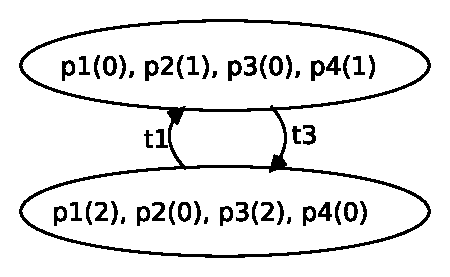
\includegraphics[scale=0.7]{Erreichbarkeitsgraph7-3-5.pdf}
\caption{Reversibles Netz}
\end{figure}

\section*{Aufgabe 7.5}

\end{document}